\documentclass[10pt]{beamer}

\mode<presentation> {

% \usetheme{Berlin}  % Squares
\usetheme{Madrid}  % Circles & dense
% \usetheme{Frankfurt}  % Cirles

\setbeamertemplate{headline}{%
\leavevmode%
  \hbox{%
    \begin{beamercolorbox}[wd=\paperwidth,ht=2.5ex,dp=1.125ex]{palette quaternary}%
    \insertsectionnavigationhorizontal{\paperwidth}{}{\hskip0pt plus1filll}
    \end{beamercolorbox}%
  }
}

\setbeamertemplate{navigation symbols}{}  % To remove the navigation symbols from the bottom of all slides uncomment this line
\setbeamertemplate{items}[circle]

% \useoutertheme{miniframes}
% \useinnertheme{circles}

}

\usepackage{graphicx}
\usepackage{booktabs}
\usepackage{fontspec}
\usepackage{xunicode}
\usepackage{xltxtra}
\usepackage{xecyr}
\usepackage{hyperref}
\usepackage{amsthm}
\usepackage{blindtext}
\usepackage{color}
\usepackage[normalem]{ulem}
\usepackage{url}
\usepackage[font=small,labelfont=bf]{caption}
\usepackage[subrefformat=parens]{subcaption}
\captionsetup{compatibility=false}
\captionsetup[subfigure]{labelformat=empty}

\usepackage{polyglossia}
\setdefaultlanguage{russian}
\setmainfont[Mapping=tex-text]{CMU Serif}
\setsansfont[Mapping=tex-text]{CMU Sans Serif}
\setmonofont[Mapping=tex-text]{CMU Serif}

\makeatletter
\DeclareUrlCommand\ULurl@@{%
  \def\UrlFont{\ttfamily\color{blue}}%
  \def\UrlLeft{\uline\bgroup}%
  \def\UrlRight{\egroup}}
\def\ULurl@#1{\hyper@linkurl{\ULurl@@{#1}}{#1}}
\DeclareRobustCommand*\ULurl{\hyper@normalise\ULurl@}
\makeatother

\newcommand\TODO[1]{\textcolor{red}{{\Large TODO: #1}}}
\newcommand\NaN{\textcolor{red}{NaN}}

%-------------------------------------------------------------------------------
%	TITLE PAGE
%-------------------------------------------------------------------------------

\title[Определение наилучшего ответа на SO]{Определение наилучшего ответа на StackOverflow}
\author[Никита Подгузов]{
Никита Подгузов 
\texorpdfstring{\vskip0.5cm \footnotesize{Научный руководитель: Рауф Курбанов}}{}
}
\institute[СПбАУ]{Санкт-Петербургский Академический университет}
\date{30 марта 2018 года}
\begin{document}

%-------------------------------------------------------------------------------
%	PRESENTATION SLIDES
%-------------------------------------------------------------------------------

\begin{frame}
\titlepage
\end{frame}

%-------------------------------------------------------------------------------

\begin{frame}
\frametitle{Введение}
\framesubtitle{Обзор}

\begin{columns}
    \begin{column}{0.6\textwidth}
        Возможности сервисов вопросов и ответов:
        \begin{itemize}
            \item Задавать вопрос (и отмечать правильный ответ) 
            \item Отвечать на вопросы, заданные другими пользователями
            \item Голосовать за понравившиеся ответы
        \end{itemize}
    \end{column}
    \begin{column}{0.4\textwidth}
        \begin{center}
            
\includegraphics[width=0.7\textwidth]{images/yahoo_answers_logo.png} \\
            
\includegraphics[width=0.7\textwidth]{images/quora_logo.png} \\
            
\includegraphics[width=0.7\textwidth]{images/stackoverflow_logo.png}
        \end{center}
    \end{column}
\end{columns}
\end{frame}

%-------------------------------------------------------------------------------

\begin{frame}
\frametitle{Введение}
\framesubtitle{StackOverflow}

\begin{columns}
    \begin{column}{0.4\textwidth}
    	Особенности системы:
    	\begin{itemize}
			\item Узкоспециализированная
			\item Большая база вопросов
			\item Наличие кода в вопросах и ответах
    	\end{itemize}
    \end{column}
    \begin{column}{0.6\textwidth}
        \begin{center}
            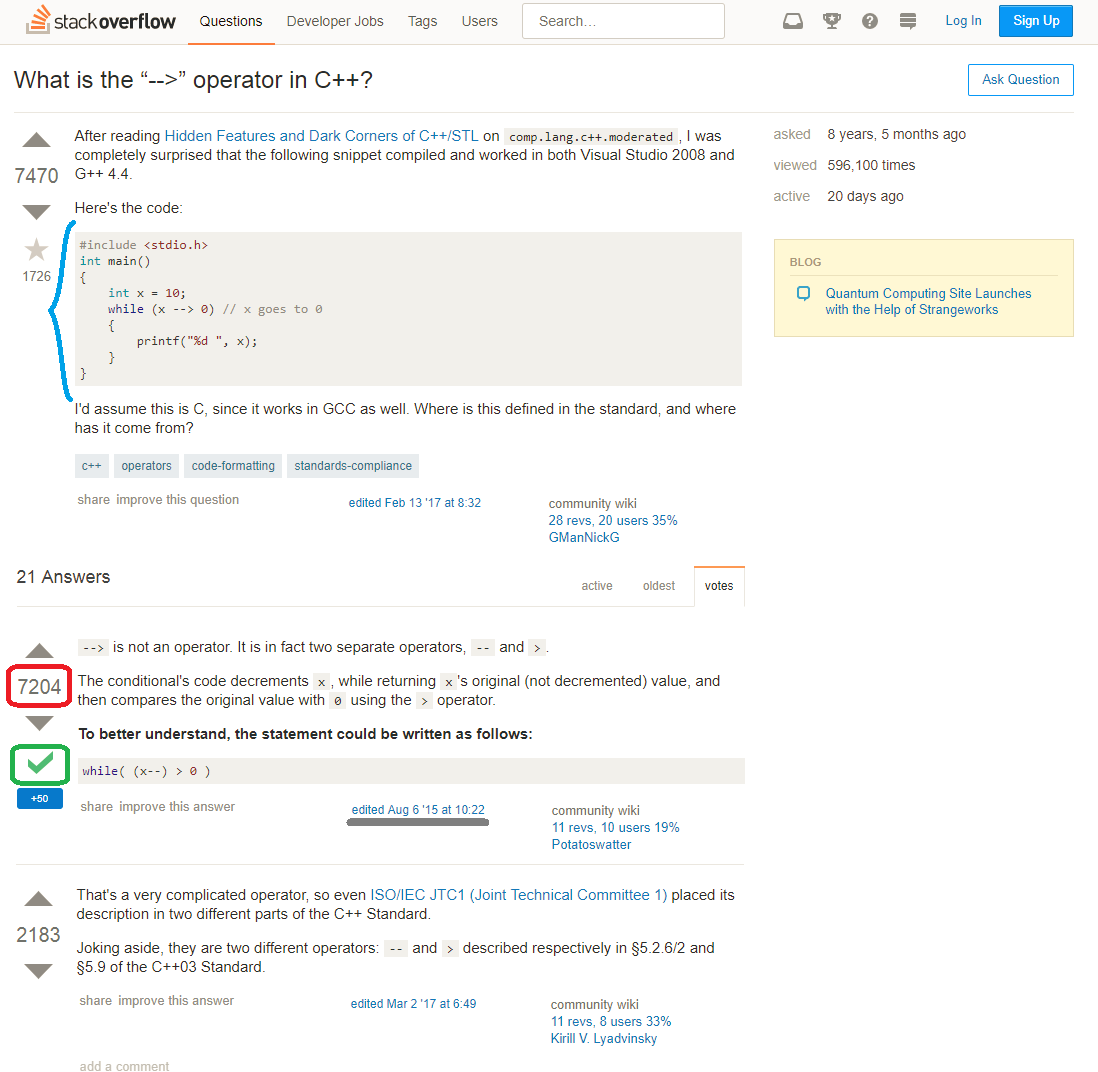
\includegraphics[width=0.95\textwidth]{images/stackoverflow_screen.png}
        \end{center}
    \end{column}
\end{columns}

\end{frame}

%-------------------------------------------------------------------------------

\begin{frame}
\frametitle{Введение}
\framesubtitle{Постановка задачи}

Проблемы:
\begin{itemize}
	\item Большая доля "неразрешенных" вопросов
	\item Нет возможности помочь оценить правильность ответов пользователю, задавшему новый вопрос
\end{itemize}

\vskip0.5cm

Хотим научиться определять правильные ответы, используя базу вопросов StackOverflow.

\end{frame}

%-------------------------------------------------------------------------------

\begin{frame}
\frametitle{Введение}
\framesubtitle{Google \& StackOverflow}

\begin{figure}
	\begin{subfigure}[b]{.49\linewidth}
		\centering
		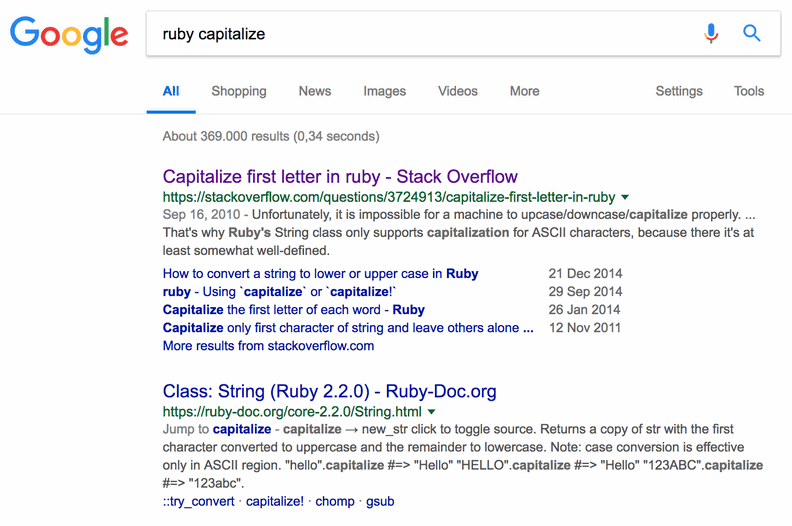
\includegraphics[width=\linewidth]{images/google_search_old.png}
		\caption{Old version}
	\end{subfigure}\hfill
	\begin{subfigure}[b]{.49\linewidth}
		\centering
		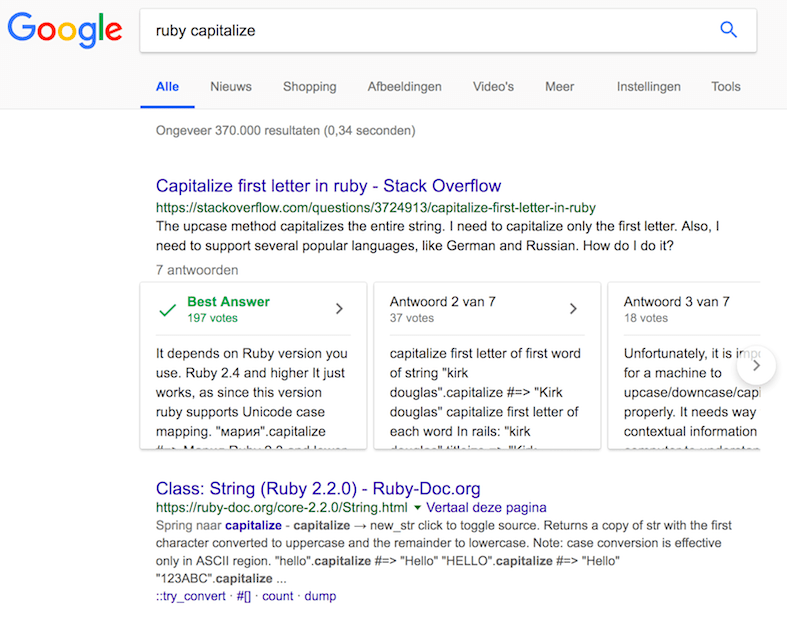
\includegraphics[width=\linewidth]{images/google_search_new.png}
		\caption{New version}
	\end{subfigure}%
\end{figure}

\end{frame}


%-------------------------------------------------------------------------------

\begin{frame}
\frametitle{Введение}
\framesubtitle{Обзор имеющихся решений}

\begin{itemize}
	\item -
\end{itemize}

\end{frame}


%-------------------------------------------------------------------------------
%	END PRESENTATION SLIDES
%-------------------------------------------------------------------------------

\end{document}